\hypertarget{analisis_resultado}{%
    \section{Análisis Resultado}\label{Análisis Resultado}}

\subsection{Descripción del DataFrame}

La tabla presenta una descripción del DataFrame, que incluye información sobre las columnas,
el número de valores no nulos y los tipos de datos correspondientes.
Analizando esta descripción, podemos obtener una visión general de la estructura y las características
del DataFrame.

\begin{table}[htbp]
    \centering
    \caption{Descripción del DataFrame}
    \begin{tabular}{lll}
        \hline
        \textbf{Columna} & \textbf{No Nulos} & \textbf{Tipo} \\
        \hline
        exitosos         & 839               & int64         \\
        fallidos         & 839               & int64         \\
        envios           & 839               & int64         \\
        sol1             & 839               & float64       \\
        aprobado         & 839               & int64         \\
        \hline
    \end{tabular}%
    \label{tab:descripcion_dataframe}%
\end{table}%

En la tabla \ref{tab:descripcion_dataframe}, contiene cinco columnas: exitosos, fallidos, envios, sol1 y aprobado.
Cada una de estas columnas tiene un total de 839 valores no nulos y se identifica el tipo de dato
correspondiente. Estos detalles son fundamentales para comprender la composición y las propiedades del DataFrame analizado.

\subsection{Estadísticas de la variable exitosos}

En el análisis de datos, es importante comprender las características estadísticas de las variables numéricas.
En este contexto, hemos examinado la variable exitosos y recopilado estadísticas como el recuento, la media,
la desviación estándar, los cuartiles y el sesgo. Estos valores nos proporcionan información sobre la
distribución y la tendencia central de la variable.

\begin{table}[htbp]
    \centering
    \caption{Estadísticas de la variable exitosos}
    \begin{tabular}{ll}
        \hline
        \textbf{Medida}    & \textbf{Valor}      \\
        \hline
        Count              & 839.000000          \\
        Mean               & 7.476758            \\
        Standard Deviation & 5.361101            \\
        Minimum            & 0.000000            \\
        25\% Percentile    & 3.000000            \\
        50\% Percentile    & 7.000000            \\
        75\% Percentile    & 11.000000           \\
        Maximum            & 28.000000           \\
        Skewness           & 0.18644798387069741 \\
        \hline
    \end{tabular}%
    \label{tab:estadistica_variable_exito}%
\end{table}%

En la tabla \ref{tab:estadistica_variable_exito}, la variable exitosos presenta una media de aproximadamente 7.48 y una desviación estándar de alrededor de 5.36.
La distribución de los datos muestra una ligera asimetría positiva con un sesgo de aproximadamente 0.19.
Estos resultados nos ayudan a comprender la variabilidad y la forma de la distribución de la variable exitosos.

\subsection{Coeficiente de asimetría}

El coeficiente de asimetría es una medida estadística que nos proporciona información sobre la asimetría de
una distribución de datos. En el contexto de los datos analizados, hemos obtenido un coeficiente de asimetría
de aproximadamente 0.1864. Este valor indica una ligera asimetría positiva en la distribución.

\begin{table}[htbp]
    \centering
    \caption{Coeficiente de asimetría}
    \begin{tabular}{ll}
        \hline
        \textbf{Coeficiente de asimetría}      & \textbf{Valor}      \\
        \hline
        Coeficiente de asimetría               & 0.18644798387069741 \\
        Coeficiente de asimetría en porcentaje & 18.64\%             \\
        \hline
    \end{tabular}%
    \label{tab:skewness}%
\end{table}%

En la tabla \ref{tab:skewness}, se puede apreciar la aproximacion de 0.1864 lo cual nos indica que la distribución de los datos tiene una
ligera asimetría hacia la derecha. Esto implica que hay una cola derecha más larga en comparación con la
cola izquierda de la distribución. En términos porcentuales, esta asimetría representa aproximadamente
el 18.64\% del rango total de la distribución.

\subsection{Coeficiente de Variación}

El coeficiente de variación es una medida de la dispersión relativa de una variable en relación a su media.
Nos permite evaluar la variabilidad de los datos en comparación con su valor promedio. Se calcula dividiendo
la desviación estándar por la media y se expresa como un porcentaje.

\begin{table}[htbp]
    \centering
    \caption{Coeficiente de Variación}
    \begin{tabular}{ll}
        \hline
        \textbf{Medida}                        & \textbf{Valor}     \\
        \hline
        Coeficiente de Variación               & 0.7166080688736847 \\
        \hline
        Coeficiente de Variación en Porcentaje & 71.66\%            \\
        \hline
    \end{tabular}
    \label{tab:coef_variacion}
\end{table}

En la tabla \ref{tab:coef_variacion}, se muestra el coeficiente de variación calculado para los
datos analizados. El coeficiente de variación es de aproximadamente 0.7166, lo que indica una alta
dispersión relativa en relación con la media. Esto se confirma por el coeficiente de variación en porcentaje,
que es del 71.66\%. Estos resultados destacan la variabilidad de los datos en el conjunto de datos analizado.

\subsection{Obteniendo Amplitud}

La amplitud es una medida de la variabilidad o dispersión de los datos. Nos permite evaluar la diferencia
entre el valor máximo y mínimo de una variable, proporcionando información sobre la extensión de los datos
en el conjunto.

\begin{table}[htbp]
    \centering
    \caption{Amplitud}
    \begin{tabular}{ll}
        \hline
        \textbf{Medida} & \textbf{Valor}     \\
        \hline
        Amplitud        & 2.6137110795050504 \\
        \hline
    \end{tabular}
    \label{tab:amplitud}
\end{table}

En la tabla \ref{tab:amplitud}, se muestra la amplitud calculada para los datos analizados. La amplitud es de
aproximadamente 2.6137, lo que indica la diferencia entre el valor máximo y mínimo de la variable.
Esta medida nos proporciona una idea de la extensión de los datos en el conjunto analizado.

\subsection{Tabla de Frecuencias}

Utilizando los datos obtenidos de la tabla \ref{tab:skewness} y la tabla
\ref{tab:amplitud}, se ha construido una tabla de frecuencias que muestra la
distribución de los datos en intervalos. Los intervalos se definen con base en la
amplitud y el valor máximo de los datos analizados.

\begin{table}[ht]
    \centering
    \caption{Tabla de Frecuencias}
    \begin{tabular}{|l|l|l|l|l|}
        \hline
        \textbf{Intervalo} & \textbf{f\_i} & \textbf{F\_i} & \textbf{h\_i} & \textbf{H\_i} \\
        \hline
        (0.0, 2.61]        & 24            & 24            & 0.028605      & 0.028605      \\
        (2.61, 5.22]       & 96            & 120           & 0.114422      & 0.143027      \\
        (5.22, 7.83]       & 128           & 248           & 0.152563      & 0.295590      \\
        (7.83, 10.44]      & 161           & 409           & 0.191895      & 0.487485      \\
        (10.44, 13.05]     & 135           & 544           & 0.160906      & 0.648391      \\
        (13.05, 15.66]     & 48            & 592           & 0.057211      & 0.705602      \\
        (15.66, 18.27]     & 69            & 661           & 0.082241      & 0.787843      \\
        (18.27, 20.88]     & 1             & 662           & 0.001192      & 0.789035      \\
        (20.88, 23.49]     & 1             & 663           & 0.001192      & 0.790226      \\
        (23.49, 26.1]      & 3             & 666           & 0.003576      & 0.793802      \\
        \hline
    \end{tabular}
    \label{tab:tabla_frecuencias}
\end{table}

En la tabla \ref{tab:tabla_frecuencias}, se presenta la tabla de frecuencias que
muestra la cantidad de datos en cada intervalo, el total acumulado de datos hasta ese
intervalo, la frecuencia relativa del intervalo y la frecuencia relativa acumulada.
Esta tabla nos permite visualizar la distribución de los datos y su acumulación en cada
intervalo.

El intervalo más relevante en esta tabla es el intervalo (7.83, 10.44], ya que contiene
la mayor frecuencia (161) y la mayor acumulación (409). Esto indica que la mayoría de
los datos se encuentran en este rango de valores.

\subsection{Histograma con curva de densidad}

El histograma con curva de densidad es una herramienta visual importante en el análisis de datos
para comprender la distribución de los valores de la variable Exitosos.

\begin{figure}[ht]
    \centering
    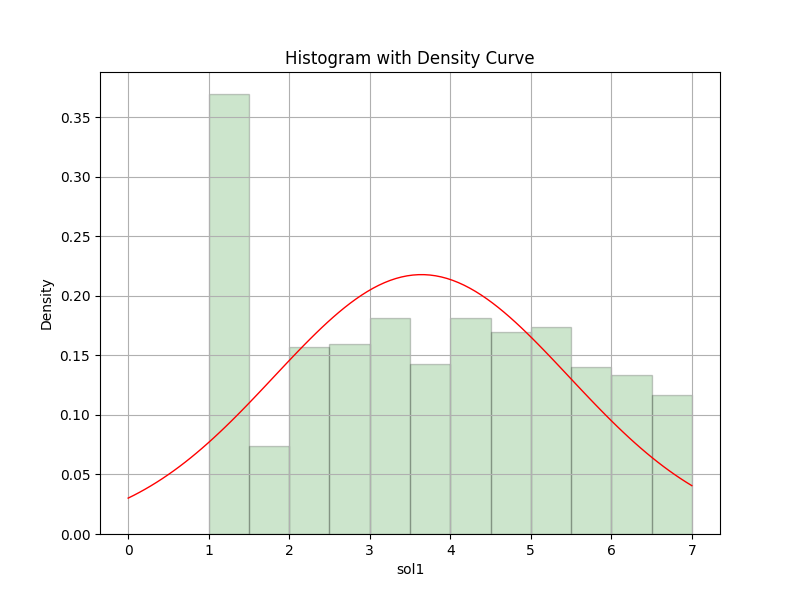
\includegraphics[width=4.06111in,height=2.68611in]{img/histogramaConCurvaDeDensidad.png}
    \caption{Histograma con Curva de Densidad}
    \label{fig:hist_density}
\end{figure}

La figura \ref{fig:hist_density} muestra este tipo de gráfico correspondiente a los datos analizados.

El eje Y muestra la densidad en el rango de 0.00 a aproximadamente 0.08, mientras que el eje X
representa la cantidad de éxitos de 0 a 25. La mayor concentración de la distribución se
encuentra alrededor de 0.08 en el eje Y y 0 en el eje X, lo cual indica que la mayoría de
las observaciones tienen un número bajo de éxitos.

La curva de densidad, en color rojo, comienza cerca de (0.02, 0) en el eje Y y se extiende hasta
(10, 0.04) en el eje X. Esta curva suavizada muestra la forma general de la distribución de los
valores de Exitosos. A medida que aumenta la cantidad de éxitos, la densidad tiende a
incrementar, lo cual se refleja en la curva que sube desde un punto cercano a 0 en el eje Y
hasta aproximadamente 0.04 en el eje X.

En resumen, el análisis del histograma con curva de densidad revela que la mayoría de las
observaciones tienen un número bajo de éxitos, con una concentración máxima alrededor de 0.08 en
el eje Y y 0 en el eje X. Además, la curva de densidad muestra una tendencia creciente a medida
que aumenta la cantidad de éxitos, alcanzando un pico cerca de 0.04 en el eje X.

\subsection{Identificar valores atípicos}

En el análisis de datos, la detección de valores atípicos es crucial para identificar
observaciones que difieren significativamente de la tendencia general. Estos valores pueden
tener un impacto significativo y requerir atención especial.

A continuación se muestra una tabla con los valores atípicos identificados mediante el método
del Z-score. Se calculó el Z-score para cada observación utilizando un umbral de 3 desviaciones
estándar.
Los valores que superan este umbral se consideran atípicos y se presentan en la tabla:

\begin{table}[ht]
    \centering
    \begin{tabular}{cccccc}
    \hline
    \textbf{exitosos} & \textbf{fallidos} & \textbf{envios} & \textbf{sol1} & \textbf{aprobado} \\
    \hline
    6 & 41 & 47 & 1.5 & 0 \\
    0 & 47 & 47 & 1.6 & 0 \\
    9 & 38 & 47 & 1.6 & 0 \\
    9 & 38 & 47 & 2.4 & 0 \\
    26 & 37 & 63 & 2.5 & 0 \\
    26 & 5 & 31 & 3.4 & 0 \\
    7 & 40 & 47 & 4.3 & 1 \\
    28 & 35 & 63 & 4.4 & 1 \\
    26 & 5 & 31 & 4.6 & 1 \\
    5 & 42 & 47 & 7.0 & 1 \\
    \hline
    \end{tabular}
    \label{tab:valores_atipicos}
    \end{table}

Observando los valores atípicos en la tabla \ref{tab:valores_atipicos}, podemos notar que algunas
observaciones difieren significativamente en al menos una de las variables. Exitosos representa
las respuestas correctas de la guía, Fallidos indica la cantidad de errores para lograr los
Exitosos, y Envíos es la suma de Exitosos y Fallidos. Sol1 se refiere a la nota
obtenida en la solemne 1.

Estos valores atípicos pueden ser de interés para un análisis más detallado, ya que podrían
indicar situaciones excepcionales o errores en la recolección de datos.